\documentclass[11pt,a4paper]{article}
\input{../../../sablony/pripravy/priprava.sty}
\usepackage{tikz}
\pagestyle{empty}
\geometry{a4paper,top=14mm,bottom=15mm,left=19mm,right=19mm}
\newcommand{\sitvelka}{%
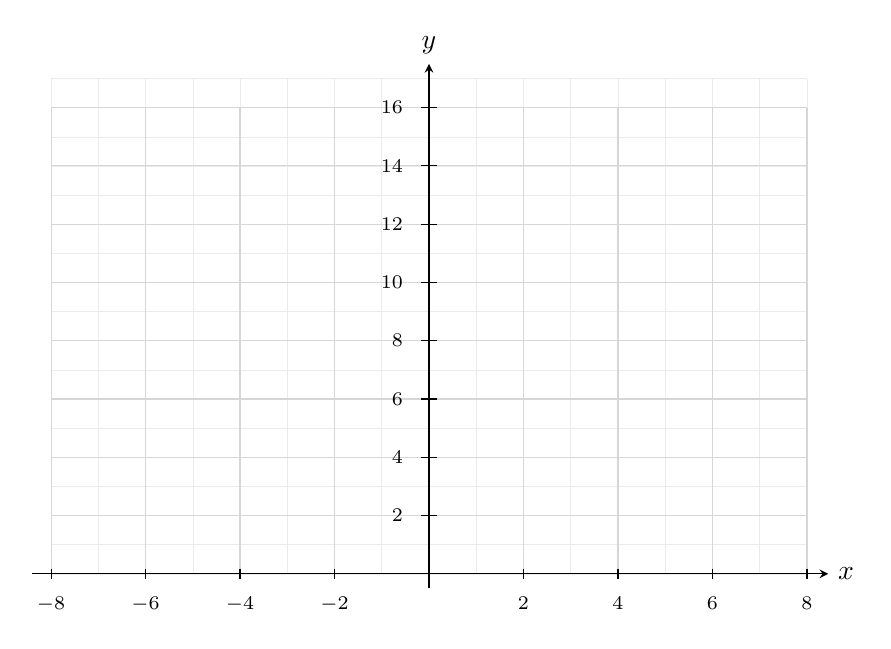
\begin{tikzpicture}[x=.60cm,y=.37cm,>=stealth]
\draw[step=1,gray!16,very thin] (-8,0) grid (8,17);
\draw[step=2,gray!32,thin] (-8,0) grid (8,16);
\draw[->] (-8.4,0)--(8.45,0) node[right] {$x$};
\draw[->] (0,-.5)--(0,17.5) node[above] {$y$};
\foreach \x in {-8,-6,-4,-2,2,4,6,8} {\draw (\x,.18)--(\x,-.18) node[below=3pt] {\scriptsize $\x$};}
\foreach \y in {2,4,6,8,10,12,14,16} {\draw (.17,\y)--(-.17,\y) node[left=3pt] {\scriptsize $\y$};}
\end{tikzpicture}}
\newcommand{\sitmala}{%
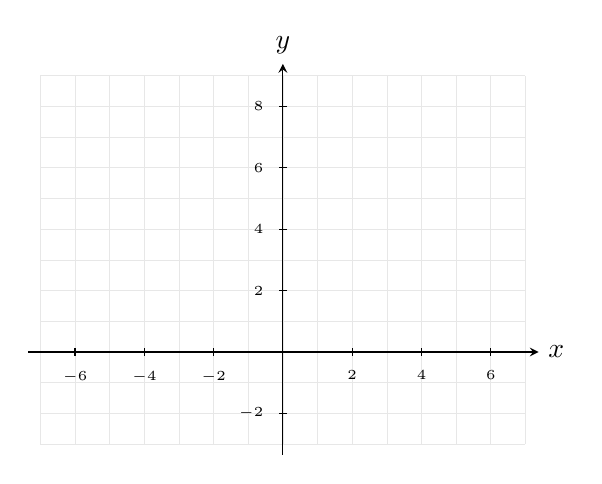
\begin{tikzpicture}[x=.44cm,y=.39cm,>=stealth]
\draw[step=1,gray!19,very thin] (-7,-3) grid (7,9);
\draw[->] (-7.35,0)--(7.38,0) node[right] {$x$};
\draw[->] (0,-3.35)--(0,9.38) node[above] {$y$};
\foreach \x in {-6,-4,-2,2,4,6} {\draw (\x,.12)--(\x,-.12) node[below=2pt] {\tiny $\x$};}
\foreach \y in {-2,2,4,6,8} {\draw (.12,\y)--(-.12,\y) node[left=2pt] {\tiny $\y$};}
\end{tikzpicture}}
\begin{document}
{\Large\bfseries Pracovní list – grafy se dvěma absolutními hodnotami}\par
\smallskip 71. hodina \hfill Jméno: \rule{66mm}{.4pt} \par
\smallskip
\textbf{Postup:} Nulové body vnitřních výrazů $\rightarrow$ intervaly $\rightarrow$ odstranění modulů $\rightarrow$ lineární části grafu. Zapiš vždy také $D(f)$ a $H(f)$.
\par\medskip
\textbf{1. Společný příklad:} $\displaystyle f(x)=|x-4|+|x+4|$.
\begin{enumerate}[label=\alph*),topsep=2pt]
\item Najdi dva body, kde se mění znaménko uvnitř absolutní hodnoty.
\item Doplň tabulku a zapiš předpis po částech.
\end{enumerate}
\renewcommand{\arraystretch}{1.28}
\begin{center}
\begin{tabular}{|l|c|c|c|}\hline
& $x<\quad\; $ & $\quad\le x\le\quad$ & $x>\quad\;$\\ \hline
$|x-4|$ & \hspace{27mm} & \hspace{27mm} & \hspace{27mm}\\[3mm]\hline
$|x+4|$ & & & \\[3mm]\hline
$f(x)$ & & & \\[3mm]\hline
\end{tabular}
\end{center}
\textbf{Předpis po částech:}\ \rule{100mm}{.4pt}\\[3mm]
\rule{155mm}{.4pt}\\[2mm]
\textbf{c) Sestroj graf a určete minimum a všechny argumenty, pro něž nastává.}
\begin{center}\sitvelka\end{center}
$D(f)=$ \rule{53mm}{.4pt}\quad $H(f)=$ \rule{59mm}{.4pt}\\[3mm]
$\min f=$ \rule{28mm}{.4pt}\qquad pro $x\in$ \rule{66mm}{.4pt}
\newpage
{\Large\bfseries Samostatné procvičování}\par\smallskip
\textbf{2.} $p(x)=|x+2|+|x-2|$. Urči $D(p),H(p)$, interval konstantnosti a načrtni graf.\\
\textbf{3.} $q(x)=|x-2|-|x+1|$. Zapiš předpis po částech, načrtni graf a urči $H(q)$.
\begin{center}
\begin{minipage}{.48\textwidth}\centering\textbf{Úloha 2}\\[2mm]\sitmala\end{minipage}\hfill
\begin{minipage}{.48\textwidth}\centering\textbf{Úloha 3}\\[2mm]\sitmala\end{minipage}
\end{center}
\textbf{Úloha 2 – předpis po částech:}\\[2mm]\rule{\linewidth}{.4pt}\\[4mm]\rule{\linewidth}{.4pt}
\medskip
\textbf{Úloha 3 – předpis po částech:}\\[2mm]\rule{\linewidth}{.4pt}\\[4mm]\rule{\linewidth}{.4pt}
\medskip
\textbf{4. Rozšíření:} $r(x)=|2x-2|+|x+2|$. Urči body změny, zapiš předpis po částech a najdi minimum. Napiš, čím se tento příklad liší od úlohy 1.\\[3mm]
\rule{\linewidth}{.4pt}\\[6mm]\rule{\linewidth}{.4pt}\\[6mm]\rule{\linewidth}{.4pt}
\end{document}
